\chapter{Methods for expert review}

Previously we have talked about what heuristics are and how they relate to usability testing. In this chapter the focus is on finding a set of applicable heuristics for evaluating video game tutorials, and constructing a set of heuristics from that pool to use in our expert review. We also have to form a selection of games that will be the target of our evaluation.

\section{Building heuristics}

There are a number of papers and studies on the use of different heuristics in video game research and testing. Our problem here is that they are mostly related to the general game experience and how the game plays from "start to finish" in a sense. We have a rather specific part of a game --- the tutorial --- that we want to evaluate, and not all heuristics are applicable or specific enough to be used with the part in question. After a literature review on the topic there are a number of sources we will be using to combine our heuristics. \cite{Desurvire2004}, \cite{Federoff2002}, \cite{Pinelle2008}
The important thing here is to remember, that not all of these heuristics are applicable to tutorials, so we must dissect them a little bit, all the while keeping in mind the different types of video game genres they could be applied to. What follow are tutorial-specific compiled lists from separate heuristic guidelines for video game usability.

\begin{figure}
	\centering
	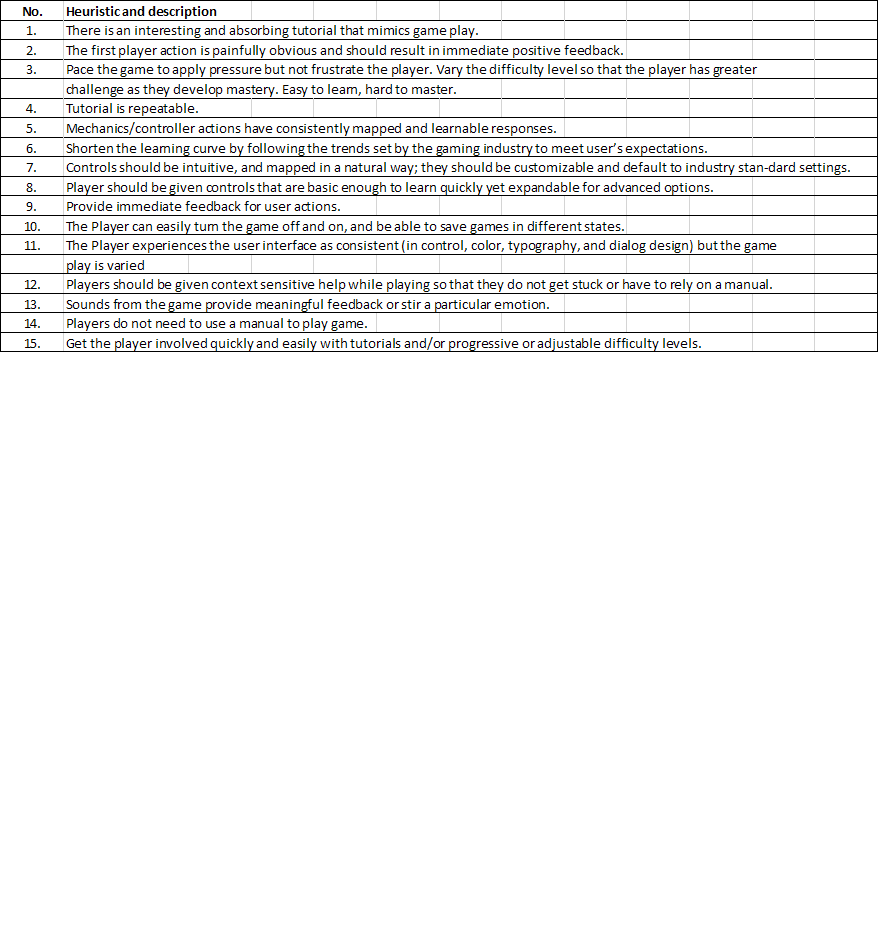
\includegraphics[width=\textwidth]{HEP}
	\caption{Tutorial-specific heuristics compiled from Desurvire et. al [2008].}
\end{figure}
\clearpage

The heuristics in Table 3.1 are from Heuristic Evaluation of Playability (HEP) \cite{Desurvire2004}. The original HEP contains 41 heuristics in total in four categories: Game Play, Game Story, Mechanics and Usability. Tutorial-specific heuristics could be found in all categories except Game Story. 

\section{Basis for selecting applicable video games}
There needs to be some basic fundamentals for how we choose the video games we want to evaluate here in order to have a somewhat meaningful selection in relation to the results we arrive to. Based on an earlier study on video game usability testing, we can lay out the following defining criteria and go on to choose applicable games \cite{Febretti2009a}:
\begin{enumerate}
	\item To be well known, professionally-developed, succesful titles published in the last ten years (which can be a potential indicator of long term engagement).
	\item To be refereed by specialized web sites for game quality assessment.
	\item To have at least one significant usability problem that clearly emerges at some point of the gameplay.
\end{enumerate}
